%%%%%%%%%%%%%%%%%%%%%%%%%%%%%%%%%%%%%%%%%
% Short Sectioned Assignment LaTeX Template Version 1.0 (5/5/12)
% This template has been downloaded from: http://www.LaTeXTemplates.com
% Original author:  Frits Wenneker (http://www.howtotex.com)
% License: CC BY-NC-SA 3.0 (http://creativecommons.org/licenses/by-nc-sa/3.0/)
%%%%%%%%%%%%%%%%%%%%%%%%%%%%%%%%%%%%%%%%%

%----------------------------------------------------------------------------------------
%	PACKAGES AND OTHER DOCUMENT CONFIGURATIONS
%----------------------------------------------------------------------------------------

\documentclass[paper=a4, fontsize=11pt]{scrartcl} % A4 paper and 11pt font size

% ---- Entrada y salida de texto -----

\usepackage[T1]{fontenc} % Use 8-bit encoding that has 256 glyphs
\usepackage[utf8]{inputenc}
\usepackage{fourier} % Use the Adobe Utopia font for the document - comment this line to return to the LaTeX default

% ---- Idioma --------

\usepackage[spanish, es-tabla]{babel} % Selecciona el español para palabras introducidas automáticamente, p.ej. "septiembre" en la fecha y especifica que se use la palabra Tabla en vez de Cuadro

% ---- Otros paquetes ----

\usepackage{url} % ,href} %para incluir URLs e hipervínculos dentro del texto (aunque hay que instalar href)
\usepackage{amsmath,amsfonts,amsthm} % Math packages
%\usepackage{graphics,graphicx, floatrow} %para incluir imágenes y notas en las imágenes
\usepackage{graphics,graphicx, float} %para incluir imágenes y colocarlas
\usepackage{epstopdf}
\usepackage[gen]{eurosym} %para incluir el símbolo del euro
\usepackage{cite} %para incluir citas del archivo <nombre>.bib
%\graphicspath{/images}

% Para hacer tablas comlejas
%\usepackage{multirow}
%\usepackage{threeparttable}

%\usepackage{sectsty} % Allows customizing section commands
%\allsectionsfont{\centering \normalfont\scshape} % Make all sections centered, the default font and small caps

\usepackage{fancyhdr} % Custom headers and footers
\pagestyle{fancyplain} % Makes all pages in the document conform to the custom headers and footers
\fancyhead{} % No page header - if you want one, create it in the same way as the footers below
\fancyfoot[L]{} % Empty left footer
\fancyfoot[C]{} % Empty center footer
\fancyfoot[R]{\thepage} % Page numbering for right footer
\renewcommand{\headrulewidth}{0pt} % Remove header underlines
\renewcommand{\footrulewidth}{0pt} % Remove footer underlines
\setlength{\headheight}{13.6pt} % Customize the height of the header

\numberwithin{equation}{section} % Number equations within sections (i.e. 1.1, 1.2, 2.1, 2.2 instead of 1, 2, 3, 4)
\numberwithin{figure}{section} % Number figures within sections (i.e. 1.1, 1.2, 2.1, 2.2 instead of 1, 2, 3, 4)
\numberwithin{table}{section} % Number tables within sections (i.e. 1.1, 1.2, 2.1, 2.2 instead of 1, 2, 3, 4)

\setlength\parindent{0pt} % Removes all indentation from paragraphs - comment this line for an assignment with lots of text

\newcommand{\horrule}[1]{\rule{\linewidth}{#1}} % Create horizontal rule command with 1 argument of height


%----------------------------------------------------------------------------------------
%	TÍTULO Y DATOS DEL ALUMNO
%----------------------------------------------------------------------------------------

\title{
\normalfont \normalsize
\textsc{\textbf{Ingeniería de Servidores (2016-2017)} \\ Grado en Ingeniería Informática \\ Universidad de Granada} \\ [25pt] % Your university, school and/or department name(s)
\horrule{0.5pt} \\[0.4cm] % Thin top horizontal rule
\huge Memoria Práctica 1 \\ % The assignment title
\horrule{2pt} \\[0.5cm] % Thick bottom horizontal rule
}

\author{Adrián Morente Gabaldón} % Nombre y apellidos

\date{\normalsize\today} % Incluye la fecha actual

%----------------------------------------------------------------------------------------
% DOCUMENTO
%----------------------------------------------------------------------------------------

\begin{document}

\maketitle % Muestra el Título

\newpage %inserta un salto de página

\tableofcontents % para generar el índice de contenidos

\listoffigures

\listoftables

\newpage

%----------------------------------------------------------------------------------------
%	Cuestión 1
%----------------------------------------------------------------------------------------

\section{¿Qué modos y/o tipos de virtualización existen? (no más de tres párrafos)}

\begin{itemize}
	\item \textbf{Virtualización asistida por Hardware}: consiste en incluir extensiones en la arquitectura del procesador de 32 bits para permitir al software
	la virtualización. En esta arquitectura, podemos diferenciar cuatro diferentes privilegios de ejecución, del 0 al 3, inversamente proporcional en cuanto a
	privilegios; siendo 0 el nivel en el que se ejecutan las operaciones del kernel. En este caso, añadiríamos un nuevo anillo con valor \emph{-1}, que actuará
	como hipervisor para aislar a la virtualización del resto de capas software.
		
	\item \textbf{Virtualización de almacenamiento}: supone abstraernos del almacenamiento físico para tratar todos los volúmenes como lógicos. Se suele usar en
	sistemas como \emph{SANs (Storage Area Network}, Red de área de almacenamiento), que consisten en grandes arquitecturas con un gran número de discos duros
	conectados mediante una red de alta velocidad. Este tipo de virtualización permite gestionar dichos volúmenes de almacenamiento de forma unitaria y más cómoda,
	tratando a todo el \emph{storage pool} como si de un solo volumen lógico se tratase.
	
	\item \textbf{Particionamiento}: es un recurso muy utilizado de forma cotidiana, como tenemos la mayoría de los alumnos de Informática, para posibilitar la 
	instalación de dos sistemas operativos. Consiste en dividir un solo recurso de gran tamaño, como puede serlo un disco duro, en recursos más pequeños y del 
	mismo tipo.
	
	\item \textbf{Máquina virtual}: esta es otra herramienta muy usada comúnmente, ya sea para la utilización de sistemas operativos en un sistema sin alojarlo
	en el disco duro directamente, o para levantar servidores sobre ella. Se montan sobre el hardware y dispositivos físicos, aunque su funcionamiento se abstrae
	de dichos componentes.
\end{itemize}


\section{Muestre los precios y características de varios proveedores de VPS (Virtual Private Server) y compare con el precio de servidores
	dedicados (administrados y no administrados). Comente diferencias.}

Para amenizar el estudio, me ceñiré a analizar solo la oferta cuyo precio coincida con el del resto de proveedores. Por ejemplo, en el primer caso
solo veremos ofertas de 15\euro{}, para poder valorar según rendimiento ofrecido. Además, en muchos casos veremos precios 'de inicio', ya que dentro
de un mismo presupuesto las compañías ofrecen algunas características más añadiendo un suplemento en el precio. \\

Entre los VPS administrados he encontrado proveedores como STRATO, AlojaRed y Contabo; los cuales ofrecen, respectivamente:
\begin{itemize}
	\item Por 15\euro{}: 2 cores CPU, 3GB RAM y 60GB SSD \cite{strato}
	\item Por 15\euro{}: 4 cores CPU, 8GB RAM y 400GB SSD \cite{alojared}
	\item Por 15\euro{}: 6 cores CPU, 24GB RAM y 600GB SSD \cite{contabo}
\end{itemize}
En este caso, el mejor proveedor según relación calidad/precio sería Contabo. Además, cabe destacar que es el único que destaca en su página web que
utiliza procesadores Intel Xeon, mientras que los otros dos no especifican nada. \\

Entre los VPS no administrados he encontrado proveedores como Axarnet, 1\&1 y ADW; los cuales ofrecen, respectivamente:
\begin{itemize}
	\item Por 15\euro{}: 4 cores CPU, 6GB RAM y 100GB SSD \cite{axarnet}
	\item Por 15\euro{}: 2 cores CPU, 4GB RAM y 120GB SSD \cite{1and1}
	\item Por 15\euro{}: 6 cores CPU, 8GB RAM y 150GB SSD \cite{adw}
\end{itemize}
Aunque encontramos unas configuraciones muy similares, solo Axarnet asegura el uso de procesadores Intel Xeon.

Dentro de los servidores dedicados, para unificar la búsqueda usaré ofertas en torno a los 160\euro{}, ya que es el resultado más encontrado en casi
todos los proveedores (aunque hay ofertas mucho más caras con muy altas prestaciones). \\

Entre los servidores dedicados administrados he encontrado proveedores como Acens, Hostalia y Dinahosting; que ofrecen respectivamente:
\begin{itemize}
	\item Por 160\euro{}: 4 cores CPU, 32GB RAM (máx.) y 2TB HDD (y 200/400/800GB SSD pagando un suplemento) \cite{acens}
	\item Por 160\euro{}: 4 cores CPU, 32GB RAM (máx.) y 2TB HDD (y 200/400/800GB SSD pagando un suplemento) \cite{hostalia}
	\item Por 170\euro{}: 4 cores CPU, 64GB RAM (máx.) y 1TB HDD (y 120/480/1024GB SSD pagando un suplemento) \cite{dinahosting}
\end{itemize}
En este caso todos los proveedores usan servidores de la marca Dell, y procesadores Intel Xeon.

Entre los servidores dedicados no administrados he encontrado proveedores como Dinahosting, RubinHost y Egalan; que ofrecen respectivamente:
\begin{itemize}
	\item Por 128\euro{}: 4 cores CPU, 4GB RAM y 1TB HDD (y 120/480/1024GB SSD pagando un suplemento) \cite{dinahosting2}
	\item Por 130\euro{}: 4 cores CPU, 96GB RAM y 8TB HDD o 1TB SSD \cite{rubinhost}
	\item Por 149\euro{}: 4 cores CPU, 16GB RAM y 2TB HDD \cite{egalan}
\end{itemize}

Para concluir, vemos una pequeña tabla con la media de precios que ya hemos visto, y podemos sacar conclusiones rápidas como que
los servidores administrados son obviamente mucho más caros que los no administrados, ya que requieren una supervisión constante,
además de actualizaciones y tareas de administración (como menciona Axarnet, proveedor ya mencionado, en su página web propia:
\cite{axarnet-descripcion})

\begin{center}
	\begin{tabular}{| c | c | c|}
	\hline
	 COMPARACIÓN (euros) & Administrado & No administrado \\ \hline
	 Virtual Private Server & ~ 15 & ~ 15 \\ \hline
	 Servidor dedicado & ~ 160 & ~ 140 \\ \hline
	\end{tabular}
\end{center}


\section{a) Enumere y explique brevemente al menos tres de las innovaciones en Windows Server 2016 y 2012 R2 respecto a 2008R2.
b) ¿Qué es Windows Server 2016 nano?}

\subsection{a) Innovaciones de Windows Server}
Como describe Microsoft en su página web oficial \cite{microsoft-ws}, cada versión de Windows Server ha ido incorporando nuevas
prestaciones a su sistema operativo orientado a servidores.

Tres de las más destacadas podrían ser:
\begin{itemize}
	\item En WS2008R2 no encontramos soporte a la detección de posibles hebras para una mejor ejecución paralela de los servicios,
	mientras que en WS2012R2 y WS2016 sí.
	\item En WS2008R2 no tenemos la funcionalidad de conexión de discos, memoria y red ``en caliente'' (es decir, sin apagar la máquina)
	mientras que sí en los otros dos.
	\item EN WS2012R2 Y WS2016 encontramos una funcionalidad que mantiene los datos sin repetir en todo el sistema (salvando obviamente
	las configuraciones que implementen mirroring) y borra aquellos duplicados. Sin embargo, en WS2008R2 no está disponible.
\end{itemize}

\subsection{b) Windows Server 2016 nano}
Windows Server 2016 Nano es una opción que ha incluido Microsoft \cite{ws2016nano} en la instalación de Windows Server 2016, cuyo 
instalador, que se ejecuta sin interfaz gráfica y a partir de comandos, permite una instalación mucho más ligera, y por tanto más rápida. 
Además, requiere muchas menos actualizaciones (y reinicios)que el Windows Server en formato común. En su página web enumeran los usos a 
los que está principalmente destinado: 
\begin{itemize}
	\item Como servidor DNS,
	\item Como anfitrión para ejecución de máquinas virtuales con Hyper-V,
	\item Como anfitrión para aplicaciones que se ejecutan en la nube o en máquinas virtuales (en modo guest).
	\item Como anfitrión para Scale-Out File Server, que consiste en un servidor el cual replica todos los archivos (máquinas virtuales,
	datos, etc.) entre todos los nodos para asegurar la máxima disponibilidad y fiabilidad posible.
\end{itemize}



\section{¿Qué son los productos MAAS y Landscape ofrecidos por Canonical (la empresa que desarrolla Ubuntu)?}
\begin{itemize}
	\item \textbf{MAAS} (Metal As A Service) es una herramienta ofrecida por Canonical con vistas a gestionar los servidores físicos y clusters como si de
	máquinas virtuales en la nube se tratasen. Es decir, desde el punto de vista de la administración de sistemas, en lugar de enfrentarnos
	a cada servidor de manera individual, con el uso de MAAS podemos poner una capa de abstracción y gestionarlos de forma cómoda y unitaria.
	Con MAAS podemos levantar/tirar nodos en cualquier momento, gestionarlos o indicar al sistema qué nodos queremos usar en cada momento, con la
	facilidad que tendría utilizar una máquina virtual local. \cite{maas-doc}
	\item \textbf{Landscape} es una herramienta que permite administrar de forma sencilla varias máquinas que ejecutan Ubuntu. Es decir, con una sencilla
	aplicación podemos crear y/o modificar agrupaciones de máquinas, aplicar determinados cambios o instalar las últimas actualizaciones.
	Además, podemos realizar dichas tareas mientras que las máquinas están apagadas, aplicándose los cambios la próxima vez que se iniciasen.
	Por otra parte, Landscape aconseja sobre las últimas actualizaciones relativas a la seguridad, que pueden ser interesantes para las máquinas
	administradas. \cite{landscape-doc}
\end{itemize}

\section{¿Qué relación tiene esta distribución (CentOS) con Red Hat y con el proyecto Fedora?}

Red Hat es un sistema operativo dirigido por \emph{Red Hat Enterprise Linux} (RHEL), y aunque es de pago, es de código abierto. Conforme se van liberando
versiones y actualizaciones de Red Hat, la comunidad de usuarios de CentOS accede a ese código, lo modifica y lo libera (ya sea en forma de código o de
binarios) como código de CentOS \cite{centos}, añadiéndolo a su sistema operativo. Como vemos, CentOS se trata de un sistema \emph{community-driven}. 
En cambio, aunque el proyecto Fedora \cite{redhat} también está dirigido por la empresa RHEL, el código de su sistema operativo no tiene ninguna relación
con el de Red Hat (obviando que ambos implementan el kernel de Linux, claro está).


\section{¿Qué diferencias hay entre RAID mediante SW y mediante HW?}

Una configuración RAID mediante hardware supone un subsistema gestor de RAID independiente al sistema anfitrión, gestionando el RAID de forma
independiente y presentándose a la máquina anfitriona como si de un solo disco se tratase. Además, tienen la ventaja de poder conectarse y desconectarse
discos y redes ``en caliente''; es decir, sin tener que reiniciar el sistema. \\
Por otro lado, una configuración RAID basada en software se implementa como un programa directamente en el kernel, y suponen una opción mucho más barata
frente a los RAIDS vía-hardware. Al ser menos costosa, no incluye funcionalidades como la conexión ``en caliente''. Hoy en día, gracias al gran rendimiento
de las CPUs actuales, esta configuración no tiene demasiado que envidiar a la configuración hardware.
\cite{raidSW-HW}

\section{a) ¿Qué es LVM? b) ¿Qué ventaja tiene para un servidor de gama baja? c) ¿Si va a tener un servidor web, ¿le daría un
tamaño grande o pequeño a /var?}

\subsection{a) LVM}
El gestor de volúmenes lógicos permite a los administradores crear volúmenes lógicos a partir de uno o más discos físicos (ya
sean particiones RAID de cualquier tipo o discos HDD comunes). La ventaja de ésto, es que separa todo el sistema en particiones
para intentar asegurar la no pérdida de datos si ocurriera algún fallo. Un sistema organizado mediante LVM se compone de lo siguiente \cite{ubuntu-lvm}:
\begin{itemize}
	\item \textbf{Physical Volume (PV)} (volúmenes físicos): disco físico (disco duro o formato SSD) o cualquier tipo de configuración RAID.
	\item \textbf{Volume Group (VG)} (grupo de volúmenes): compuesto de uno o más volúmenes físicos. Puede extenderse mediante la inclusión
	de más discos.
	\item \textbf{Logical Volume (LV)} (volúmenes lógicos): se asemejan a las particiones corrientes. Están disponibles para su montaje y
	almacenamiento de datos, utilizando cualquiera de los conocidos formatos de archivos (ext4, XFS, JFS, etc).
\end{itemize}


\subsection{b) Ventajas de LVM para un servidor de gama baja}
La mayor ventaja que aporta LVM a la hora de instalar Linux en una máquina es la facilidad para decidir cómo queremos organizar
nuestros datos y sistemas de archivos. Podríamos comparar un servidor de gama baja con un equipo con poco espacio de disco. Por ejemplo,
si tuviéramos un disco de 20 GiB y asignásemos todo ese espacio al sistema operativo, a la hora de quedarnos sin espacio tendríamos que
sustituir el disco por uno nuevo, teniendo que reinstalar el sistema operativo para utilizar ambos discos. En cambio, con el uso de LVM
podemos particionar el primer disco separando los directorios /, /boot, /home, etc a nuestro antojo; con la ventaja de que en un futuro,
si necesitásemos añadir espacio a /home, podríamos quitarlo de otro directorio, o asignárselo en un segundo disco que adquiriésemos.

\subsection{c) Tamaño ideal para /var}
/var es el directorio del sistema en el que Linux escribe y borra constantemente datos que está utilizando en sus procesos; es por esto
que tendríamos que asignarle un espacio muy grande si destinásemos el sistema al uso de un servidor web, ya que en este directorio el sistema
operativo almacenará, leerá y borrará todas las peticiones y cuestiones con que esté trabajando.


\section{¿Debemos cifrar también el volumen que contiene el espacio para swap? ¿y el volumen en el que montaremos /boot?}
El espacio para intercambio (swap) sí debemos cifrarlo, ya que este espacio se utiliza escribiendo y moviendo datos importantes
del usuario, como pueden ser configuraciones de programas o archivos grandes con que esté trabajando en un momento en el que la memoria
física se ve afectada; y si no cifrásemos este espacio podría acceder cualquiera. \\
Por otro lado, el volumen asignado a /boot no debería ser cifrado, ya que entonces se bloquearía el gestor de arranque y no podría
iniciarse el sistema.


\section{a) Imagine que tiene un disco híbrido con tecnología SSD ¿Qué puntos de montaje ubicaría en éste? b) Justifique qué
tipo de sistema de archivos usaría para tener un servidor de streaming.}

\subsection{a) Puntos de montaje a ubicar en disco SSD}
A la hora de configurar un sistema híbrido (compuesto de discos duros y discos con tecnología SSD) habremos de ser cuidadosos con los
puntos de montaje asignados a cada disco, ya que aquellos con tecnología SSD podrían agotar sus ciclos de escritura si no tuviésemos
cuidado en este aspecto. \\
La ventaja de la tecnología SSD es principalmente su velocidad, por lo que en este tipo de discos podríamos ubicar las siguientes
particiones:
\begin{itemize}
	\item Directorio raíz (/): ya que en este punto se instalan de forma ligera todo el sistema operativo y sus programas, podremos
	aprovechar la velocidad del SSD a la hora de iniciar el sistema y ejecutar sus aplicaciones.
	\item Directorio de arranque (/boot): a este directorio se accede cada vez que se enciende el ordenador, lo que no consume prácticamente
	ciclos de escritura, y su aprovechamiento agilizaría el arranque del sistema.
\end{itemize}
Por otra parte, no deberíamos ubicar en el SSD puntos de montaje como /home o /var, ya que utilizan grandes volúmenes de memoria y
consumen muchos ciclos de lectura/escritura con la ejecución/modificación de sus archivos.

\subsection{b) Sistema de archivos para servidor de streaming}
Una vez visto un listado de los sistemas de archivos disponibles (proporcionado por The Linux Documentation Project \cite{filesystems}),
podríamos tomar como opción el sistema de ficheros \emph{NFS}, ya que está preparado para la compartición de un tipo de ficheros en red
junto con muchos otros ordenadores, permitiendo un acceso muy fácil a dichos archivos por parte de todos ellos.


\section{Muestre cómo ha quedado el disco particionado una vez el sistema está instalado y ha iniciado sesión (comando: lsblk).}
\begin{figure}[H]
	\centering
	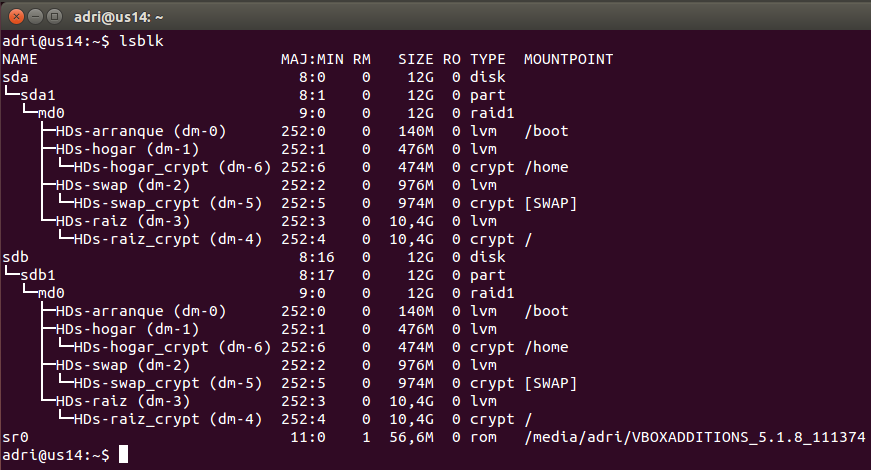
\includegraphics[scale=0.5]{lsblk-captura}
	\caption{Estado de los discos particionados visualizado desde dentro del sistema}
	\label{fig:figura1}
\end{figure}

\section{a) ¿Cómo ha hecho el disco 2 arrancable? b) ¿Qué hace el comando grub-install?}

\subsection{a) Solución para arrancar el disco 2}
A pesar de tener el segundo RAID en estado \emph{Degraded}, el sistema lo marca como \emph{Inactive}, por lo que no nos deja arrancar a partir
de él, y tras un tiempo de espera en el arranque, el sistema nos ejecuta la terminal \emph{(initramfs)}, la cual nos permitirá administrar el arranque
a modo de ultimátum. La solución consiste en acceder al fichero \emph{/proc/mdstat (mdstat = multi-device status)}, imprimir su contenido y verificar 
que efectivamente el estado del disco se muestra inactivo. \\
A continuación, para poder modificar el estado aparente del segundo disco, habremos de acceder al fichero de configuración de multidispositivos
mediante la orden \emph{mdadm -R /dev/md0}, cuyo funcionamiento explicamos a continuación:
\begin{itemize}
	\item \textbf{mdadm}: \emph{multi-device administrator},
	\item \textbf{-R}: equivale a \emph{--run} e implica forzar a la herramienta RAID a marcar el dispositivo como arrancable,
	\item \textbf{/dev/md0}: es la ruta al multi-dispositivo creado durante la instalación de Ubuntu Server.
\end{itemize} 

\begin{figure}[H]
	\centering
	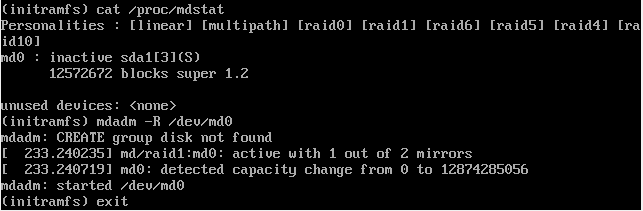
\includegraphics[scale=0.8]{mdstat-inactive}
	\caption{Demostración de la restauración de la actividad para el segundo RAID1} \label{fig:figura2}
\end{figure}

Acto seguido, ejecutamos \emph{exit} y Ubuntu Server vuelve a intentar arrancar, consiguiéndolo esta vez; cosa que comprobamos al instante ya que
nos pide las claves de cifrado convencionales.


\subsection{b) grub-install}
El comando \emph{grub-install} sirve para instalar el gestor de arranque GRUB en el volumen físico que le indiquemos como parámetro. \\
Por ejemplo, en el apartado anterior utilizamos el comando \emph{sudo grub-install /dev/sdb} para instalar un gestor de arranque en el
segundo disco RAID, para así también poder iniciar el sistema aun estando caído el primer disco.


\section{¿Qué diferencia hay entre Standard y Datacenter?}
Como la gente de Microsoft informa en su blog de Technet \cite{ws2012-versions}, no existen prácticamente diferencias técnicas entre estas dos 
versiones de Windows Server 2012R2, salvo una; que consiste en la limitación del número de máquinas virtuales que permiten sean creadas. \\
Para WS2012 Standard, su licencia restringe al uso de \underline{dos VMs como máximo}. En el caso de WS2012 Datacenter, no hay limitación en 
cuanto al uso de VMs; siendo esta la única diferencia apreciable.

\section{Continúe usted con el proceso de definición de RAID1 para los dos discos de 50MiB que ha creado. Muestre el proceso con
capturas de pantalla.}

\begin{figure}[H]
	\centering
	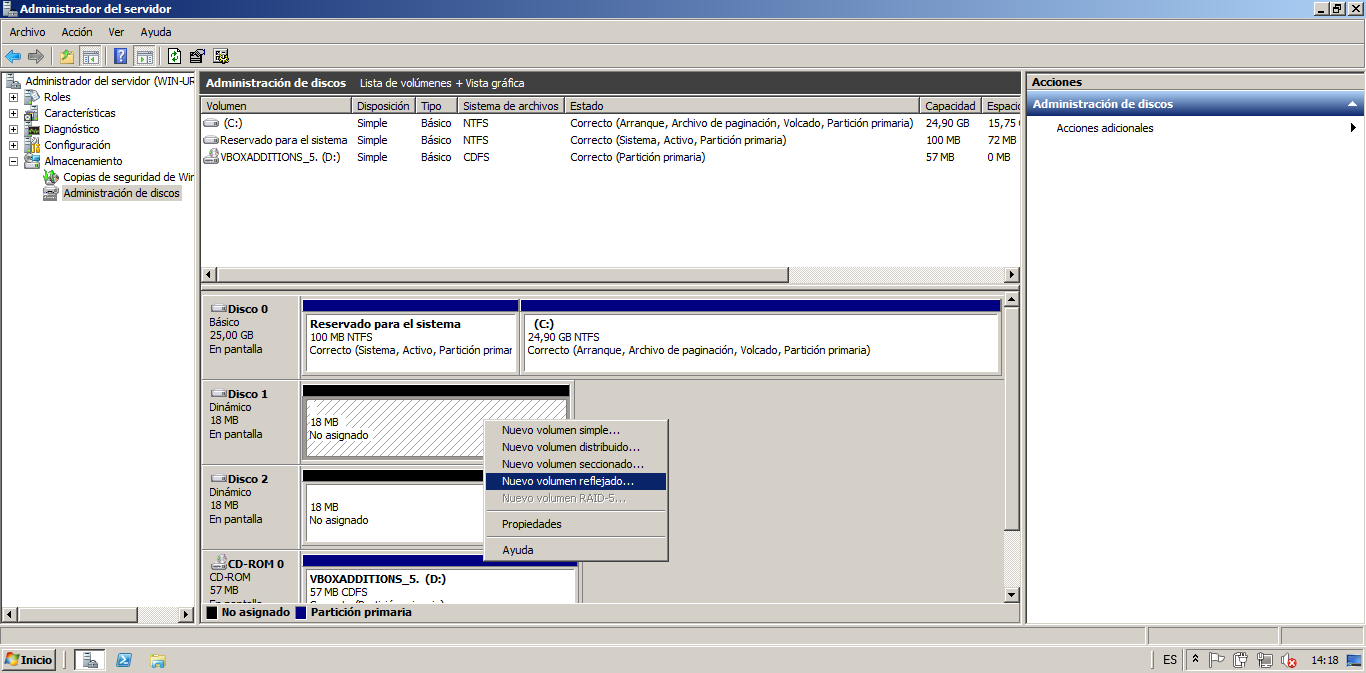
\includegraphics[scale=0.4]{WS2008-1}
	\caption{Una vez tenemos las particiones de 50MiB creadas, hacemos click derecho y elegimos la opción \emph{volumen reflejado}}
	\label{fig:figura3}
\end{figure}

\begin{figure}[H]
	\centering
	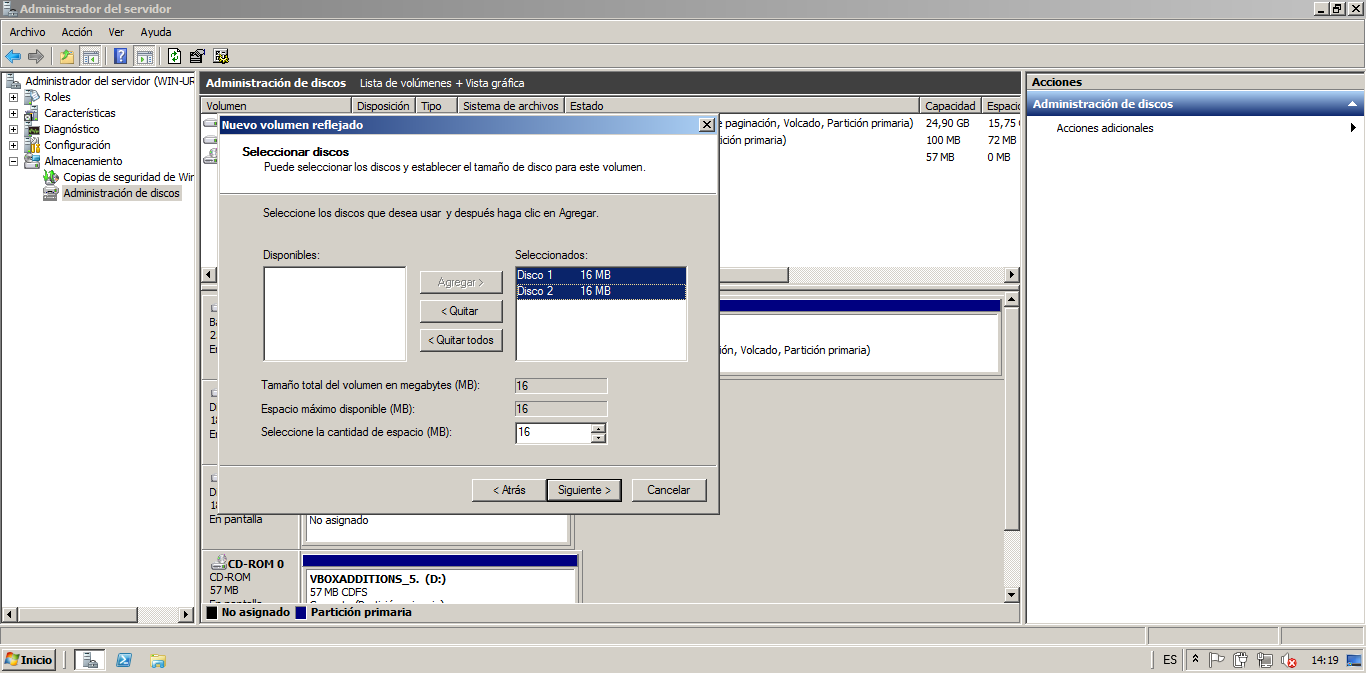
\includegraphics[scale=0.4]{WS2008-2}
	\caption{Añadimos ambos discos a la configuración RAID que tratamos de hacer}
	\label{fig:figura4}
\end{figure}

\begin{figure}[H]
	\centering
	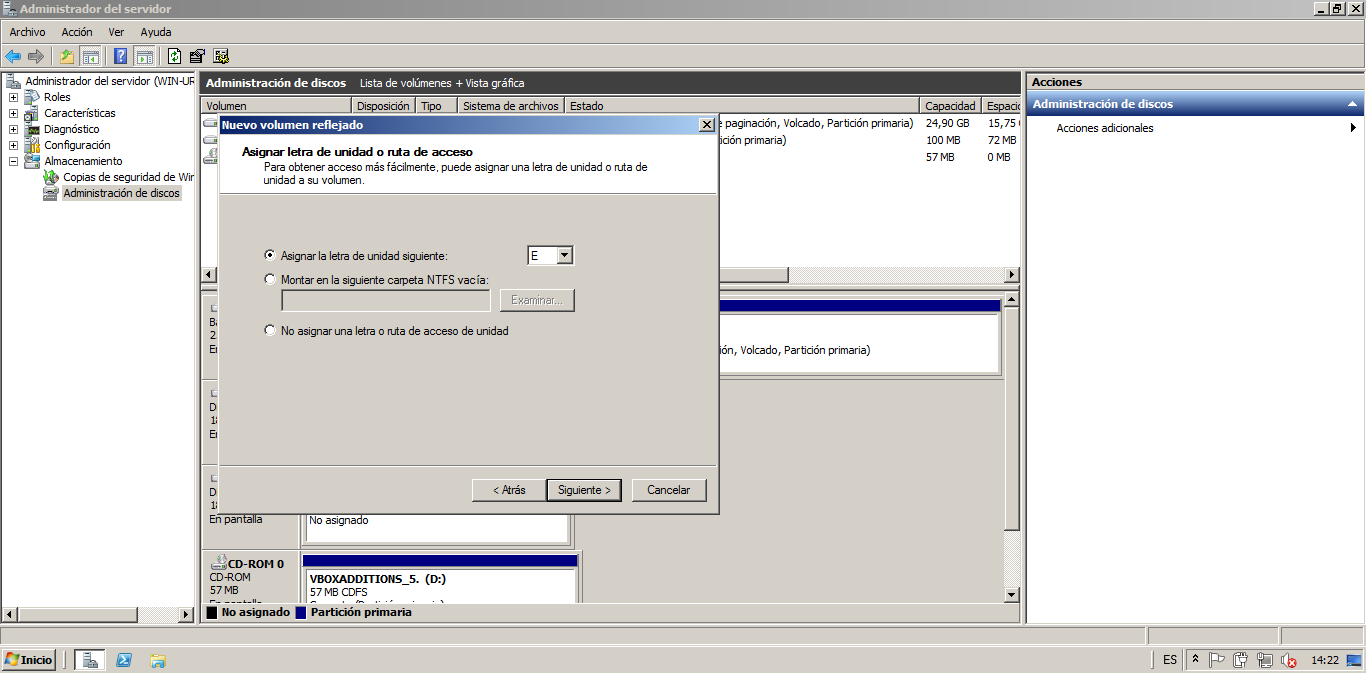
\includegraphics[scale=0.4]{WS2008-3}
	\caption{Asignamos cualquier letra de unidad (por defecto, E)}
	\label{fig:figura5}
\end{figure}

\begin{figure}[H]
	\centering
	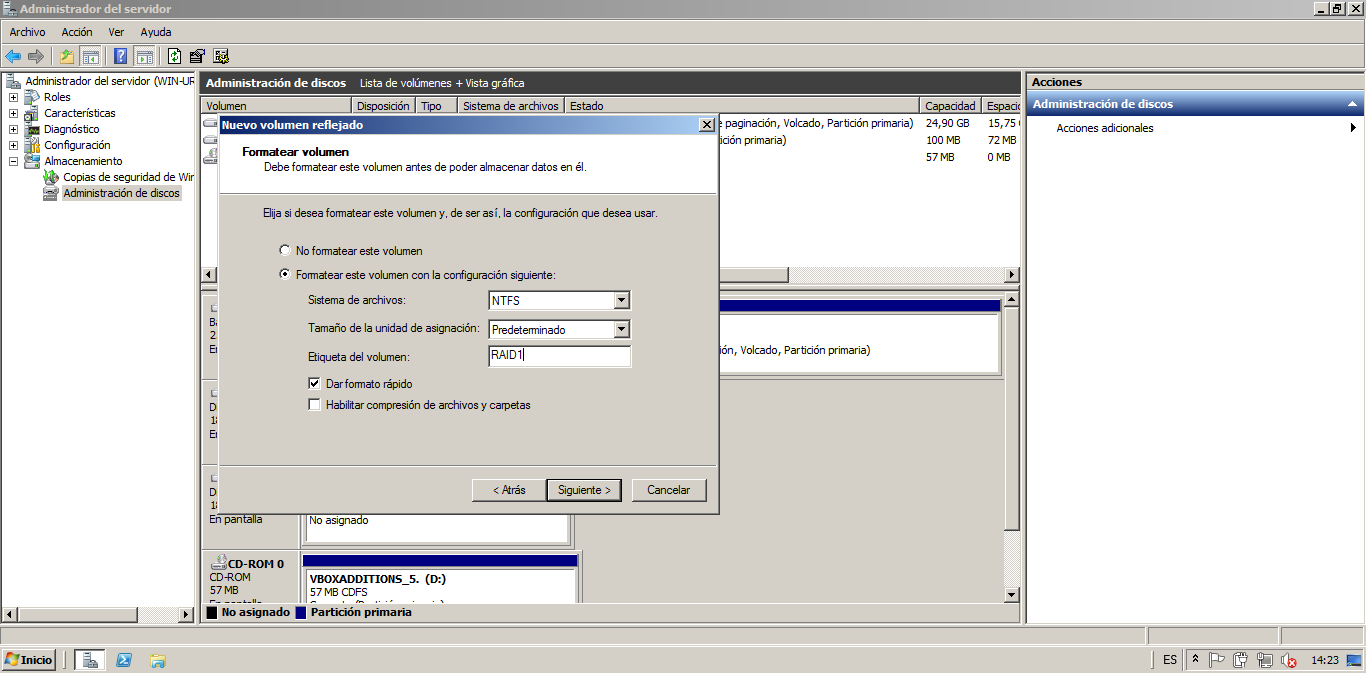
\includegraphics[scale=0.4]{WS2008-4}
	\caption{Nombramos el volumen como \emph{RAID1}}
	\label{fig:figura6}
\end{figure}

\begin{figure}[H]
	\centering
	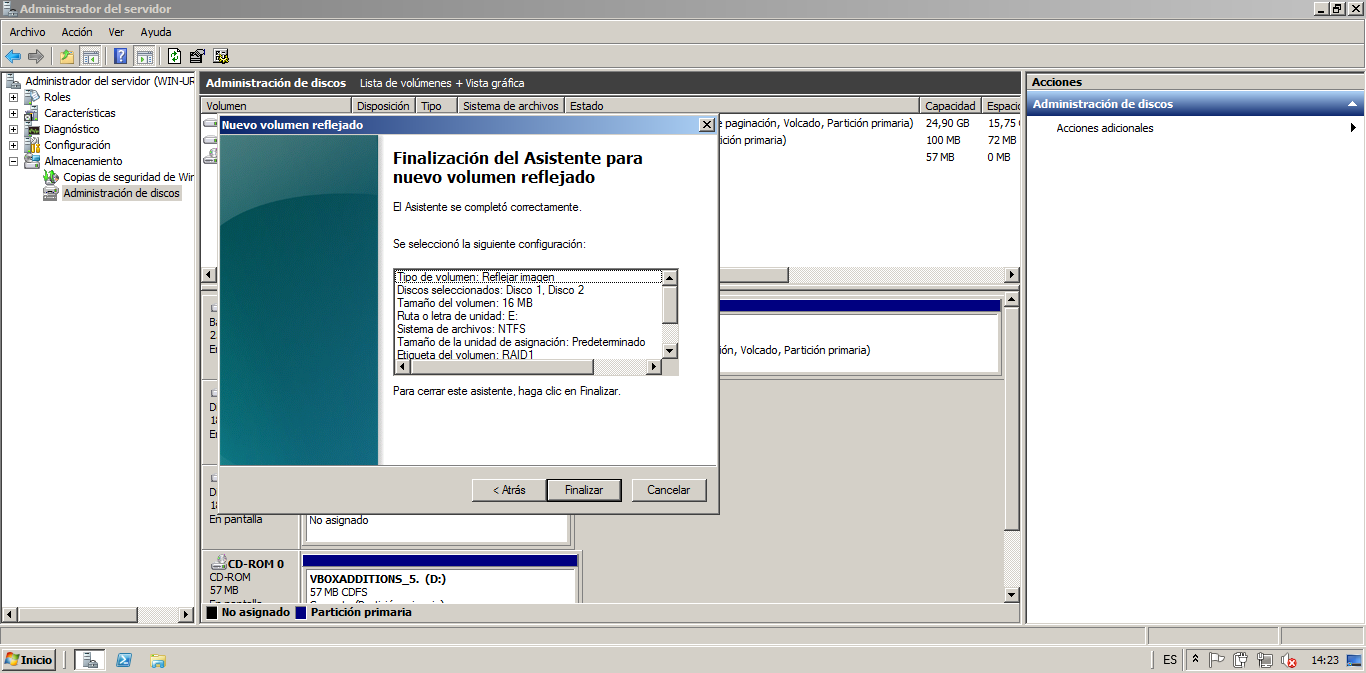
\includegraphics[scale=0.4]{WS2008-5}
	\caption{Con esto habremos terminado la instalación, pulsamos en \emph{Finalizar}}
	\label{fig:figura7}
\end{figure}

\begin{figure}[H]
	\centering
	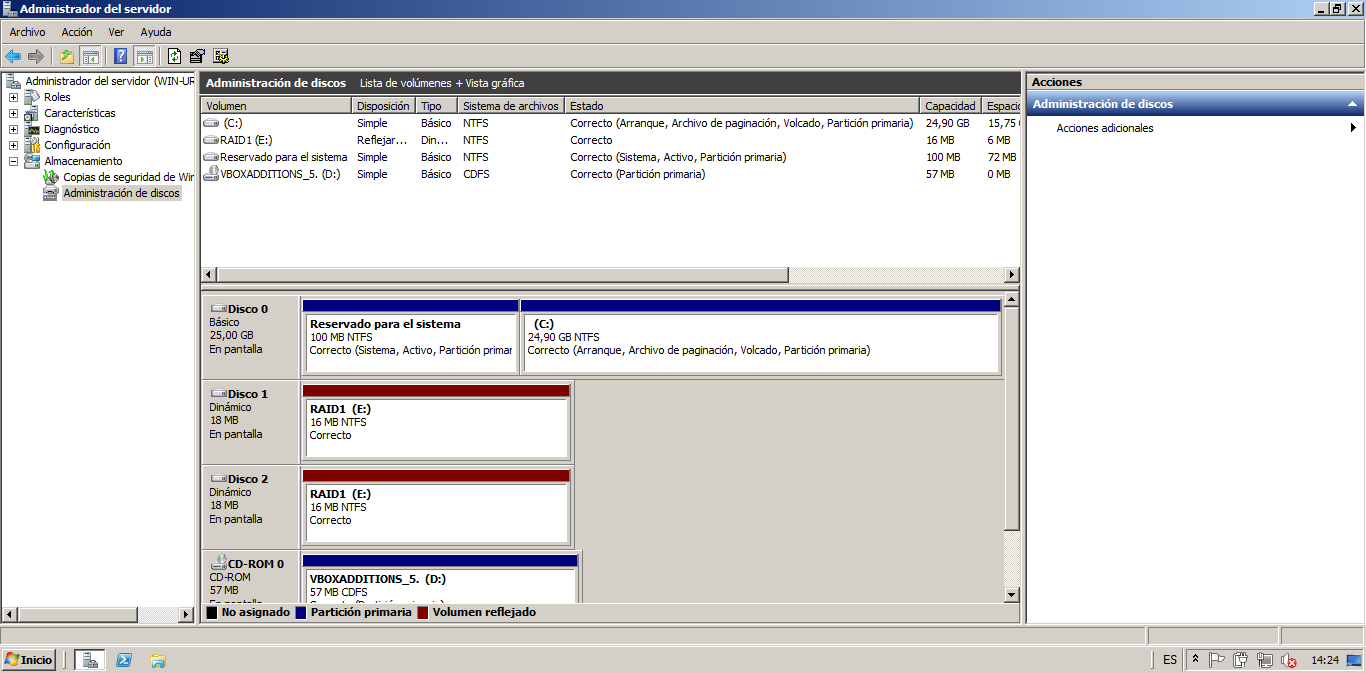
\includegraphics[scale=0.4]{WS2008-6}
	\caption{Aquí vemos finalmente la configuración de ambos discos dinámicos, configurados en modo RAID1}
	\label{fig:figura7}
\end{figure}


\section{Explique brevemente qué diferencias hay entre los tres tipos de conexión que permite el VMSW para las MVs: NAT,
Host-only y Bridge.}

Para la descripción de estos tres tipos de conexión, usaremos la herramienta Virtualbox como ejemplo, ya que es la usada en prácticas. Además, nos ayudamos de su
documentación oficial \cite{virtualbox-networks}. \\

Para empezar, la red \emph{NAT} es la que usamos cuando montamos una máquina virtual con Virtualbox, por ejemplo. El sistema anfitrión comunica al invitado a través
de la interfaz de red proporcionada por la herramienta de virtualización, sin necesidad de configurar nada ni en el sistema invitado ni en el principal. Se asemeja
a una conexión común a un router, actuando como tal la herramienta de virtualización. \\

Por otro lado, mediante la conexión \emph{Bridge}, Virtualbox comunica la red de la máquina anfitriona con la red del invitado mediante un driver hardware (\emph{
Bridged Networking} -> \emph{conexión puenteada}). Esto permite a Virtualbox filtrar todos los datos que llegan a la máquina anfitriona, creando una nueva interfaz de
red mediante software. Cuando el invitado se conecta a esta nueva interfaz, figura como conectado físicamente al sistema principal, y por tanto a la red Internet real. \\

Para terminar, el tipo de conexión \emph{Host-only} define algo similar a una red de conexiones \emph{Bridge} pero que solo comunican al anfitrión con todas las
máquinas virtualizadas, siendo éstas no visibles desde fuera de este contexto. \\

La mayor diferencia entre ambas, es que mediante conexiones \emph{NAT} y \emph{Host-only}, las máquinas virtualizadas no son accesibles desde el 
exterior (resto de Internet), mientras que con una conexión del tipo \emph{Bridge}, sí.


\bibliography{citas}
\bibliographystyle{plain}
\end{document}
